%!TEX TS-program = LuaLaTeX
\documentclass[tikz,border=0.5cm]{standalone}

\pdfvariable suppressoptionalinfo \numexpr32+64+512\relax

\begin{document}
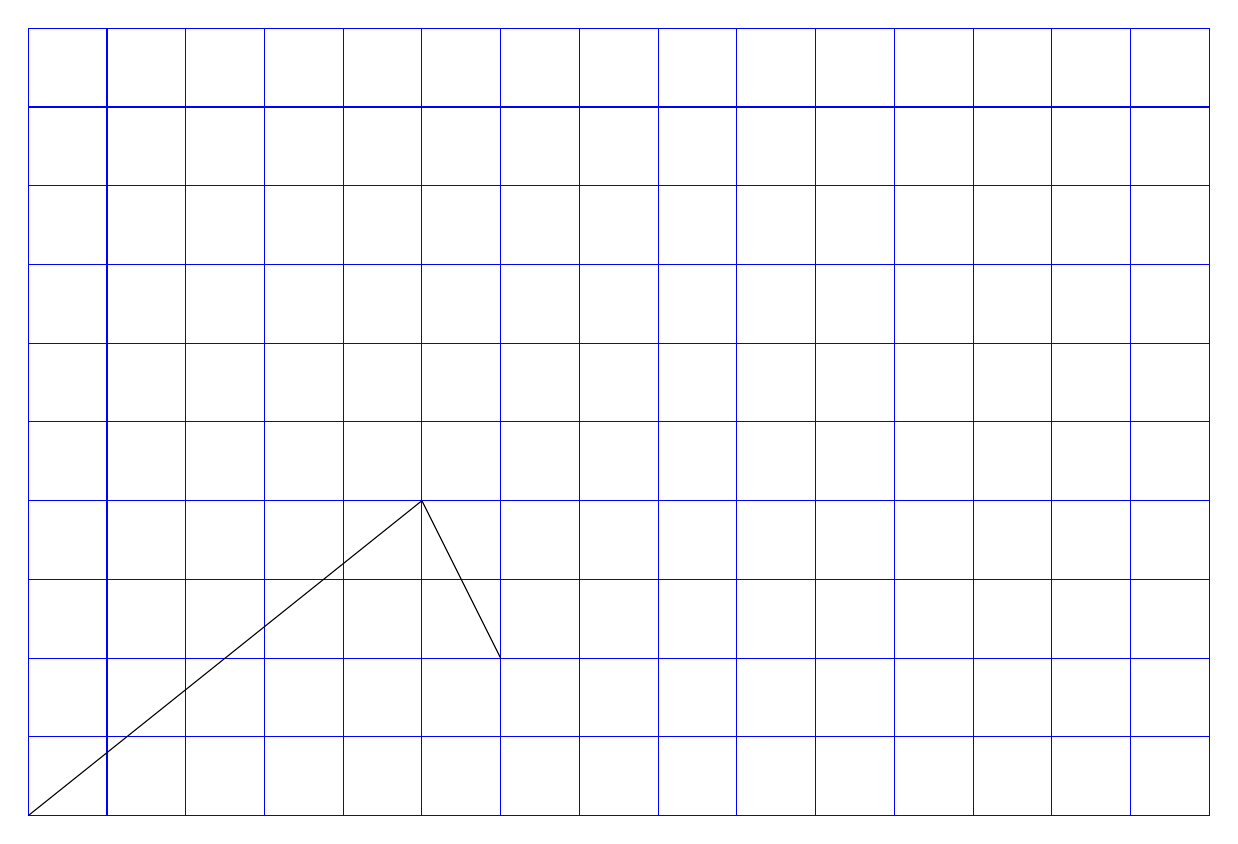
\begin{tikzpicture}
\draw[step=1cm,blue,thin] (0,0) grid (15,10);

\coordinate (a) at (0,0);
\coordinate (b) at (5,4);
\coordinate (c) at (6,2);

\draw (a) -- (b)--(c);

\end{tikzpicture}
\end{document}
 